\documentclass{article}
\usepackage{acl2012}
\usepackage{times}
\usepackage{tabularx}
\usepackage{latexsym}
\usepackage{amsmath}
\usepackage{multirow}
\usepackage{graphicx}
\usepackage{hyperref}

\DeclareMathOperator*{\argmax}{arg\,max}
\setlength\titlebox{6.0cm}    % Expanding the titlebox

\title{{\small CS224U Project} \\ Tree Conversation Reconstruction in Modern Online Discussions \\ \small{Final Report}}
\author{Julius Cheng \\
  {\tt juliusc@stanford.edu}
  \\\And
  Thomas Dimson  \\
  {\tt tdimson@cs.stanford.edu}
  \\\AND
  Milind Ganjoo \\
  {\tt mganjoo@stanford.edu}
}
\date{}
\begin{document}
\maketitle
\begin{abstract}
This paper investigates the problem of conversation disentanglement within
modern online discussion forums, which are characterized by their complex
branching structure and frequent change of topic. We present a probabilistic
model to reconstruct message trees from a flattened representation. Using a
set of novel evaluation metrics, we achieve above-baseline performance on a
new corpus of conversations from the popular Hacker News website. We also
analyze the limitations of our model, and present aspects of the
disentanglement task that could inform further research.
\end{abstract}

\section{Introduction}
Our project focuses on conversation disentanglement, which broadly refers to
the problem of guessing the structure of a multi-party, asynchronous
conversation. In particular, we discuss the problem of \textit{conversation
reconstruction}, where machine-learning is employed to recover a lost
relationship between messages.

We analyze modern internet forums such as
\textit{Hacker News}\footnote{\url{http://news.ycombinator.com}} 
and \textit{Reddit}\footnote{\url{http://www.reddit.com}}, where conversations
are represented and displayed in the user interface as trees, multiple
replies can be made to the same message, and discussions are usually sorted by
the sum of votes of approval or disapproval from other users. In
such forums, users are able to seed a conversation tree by posting a
\textit{root message}, and participants reply and begin sub-discussions
underneath this root. The forums are characterised by a complex discussion
tree that emerges as conversations drift and sub-discussions form.

In our conversation reconstruction task, we analyze a time-ordered list of
messages and construct a candidate conversation tree, presumed to be the
structure that was lost. On a high level, we minimize the reconstruction error
when forum conversation trees flatten into lists.

Some of the questions our research aims to discuss include:
\begin{itemize}
  \item To what degree does semantic knowledge allow a machine to understand the 
    flow of online forum discussions?
  \item How much does non-semantic information, such as timestamps and poster karma,
    aid the system?
  \item Does performance vary across domains? Do factors such as tree depth,
    length of messages, and similarity of messages affect our ability to
    reconstruct conversations? 
\end{itemize}

As we show, answering these questions correlates to the performance of a system
in the conversation reconstruction task. 

We have made the code and datasets for our project available online
\footnote{\url{https://github.com/cosbynator/discussion-disentanglement-cs224u}} on the
GitHub web hosting service.

\section{Prior Work}
\label{sec:prior_work}
While there has been prior work in conversation reconstruction, none examine
our exact sub-domain. There is a general divide between authors who examine
traditional online forums, where messages are long but exhibit a linear reply
structure, and authors who examine reconstruction in the context of internet
chat, where messages are relatively short and directed. Approaches taken by
authors also vary considerably: some employ rule-based systems \cite{Wang2008a}, while others
choose heavily probabilistic models such as conditional random fields. In
certain cases, conversation reconstruction has been an explored as an
evaluation metric for unsupervised models that discover \textit{speech acts}
in conversational data.

\newcite{Wang2011a} employ machine
learning to aid in the task of conversation disentanglement; in particular,
they use conditional random fields for link prediction. A crucial component of
this task is defining a set of features that capture dependencies between
posts. The paper describes two categories of features. The first kind depend
only on attributes drawn from a pair of posts, such as content similarity
score, recency, author name reference, and indicator variables that give
special importance to posts made last or first in a given thread. The second
kind also consider the parent assignments of the posts, which allows scoring
of characteristics like the similarity between  post and the \emph{parent} of
another post to determine content propagation, or accord importance to posts
that reply to the same author and are also written by the same author (which
is indicative of friends carrying out a back-and-forth conversation in a
thread). In our paper, we focus on the first kind of features that depend on
pairwise attributes only.

Similarly, in \newcite{Aumayr2011a}, the authors attempt machine learning to
tackle the problem of reconstructing conversation trees in a traditional
vBulletin-powered online forum. The authors report their best results using
C4.5-style decision trees based on classifying whether pairs of posts are in a
$(parent, child)$ relationship or not. As in our approach, their features are
a mix of shallow textual and post metadata features: TF-IDF weighted text
distance, presence of quotes and a user's name, post-distance and time
difference. Unlike in our findings, post distance is their best feature, since
their domain appears to be near-linear.

In early work, \newcite{Elsner2008a} treat disentanglement as a clustering
problem between utterances. Their dataset consists of manually annotated IRC
conversations that contain information about schisms in topics and minor
digressions. Similar to most authors, they employ a machine-learning model
using a MaxEnt classifier to decide whether a given pair of utterances belongs
to the same conversation. It then attempts to cluster the utterances to
maximize the weighted accuracy of the classifier. As with much other work,
they employ pause length and message similarity as key features in their
classifier.

\newcite{Wang2009b} expands on the above study by distinguishing
\textit{context-free} and \textit{context-sensitive} message models, where the 
former refers to using data in the message alone, including word features and the
time-stamp.  This study augments a basic set of word features with author context, 
conversational context, and temporal context of a message. Author context 
refers to all other messages written by the author, and conversational context 
refers to all messages by participants in a sub-conversation, 
where the participants are determined by all other people referred to by name 
by the author of a message.  Afterward computing their features, they perform
clustering to identify different threads of conversation.

A very different approach is seen in \newcite{Mayfield2012a}, where the authors present
a model for chat disentanglement that annotates three types of information: 1) 
Negotiation labels, or whether an utterance is providing or receiving 
information, 2) sequences, or exchanges of information, and 3) threads, the 
outcome of the standard disentanglement problem. Their algorithm performs 
two passes over the data,  one in which negotiations and sequences are generated, 
followed by a pass that groups sequences together to form threads. Uniquely,
their data was hand-annotated from verbal chat meetings for a cancer support group.
They report results that occasionally beat human annotators.

Finally, some authors consider the problem of speech disentanglement as
traversing a finite state automaton between different \textit{speech acts},
such as ``question'', ``answer'' or ``statement''. Although this is a classic
problem in natural language processing, a standard extrinsic evaluation is
discourse disentanglement. \newcite{Paula} build an unsupervised
Hidden Markov Model that  maps speech acts to hidden states. They believe that
the words of a message in a conversation are generated according to language
models associated with a state or speech act. They report hidden states that
correctly correspond to speech acts, for example, a collection of question-
related pronouns and words corresponding to a speech act beginning a forum
post about a technical question. As we show in Section \ref{sec:dataset}, our
results with their model were not as successful.

\newcite{Ritter2010a} also consider unsupervised tagging of speech
acts. The paper describes an unsupervised LDA-like approach to act tagging and
utilizes Twitter \textit{conversations} for training purposes. Fittingly,
their model was evaluated extrinsically by reconstructing the original order
of a scrambled conversations in Twitter. Their model corresponds to a
generative story where words are filled by either the conversation topic, the
dialog act of the tweet or from general English.

Unlike other speech act papers, \newcite{Kim2012} focuses on classifying
utterances in multi-party chat scenarios. The basic unit of analysis is a
contiguous message written by an individual. The authors define several
classes of features, then runs various classifiers on combinations of them.
The features include TF-IDF and unigrams, with and without stemming and
lemmatization.  The best performance in both datasets approaches 100\% on a
model using bag-of-words, keywords, and previous utterances, but not
structural information. The authors conclude that the failure of structural
information compared to previous works is likely due to entanglement.

\section{Dataset}
\label{sec:dataset}
Our approach differs from most of those listed in Section \ref{sec:prior_work}
by scale: we are trying to reconstruct large, complex conversations with a
unpredictable branching structures. After reviewing existing datasets, we
decided that gathering our own was the best option. We looked at two online
forums: Hacker News and Reddit. To ensure that all conversations had a long
and well formed root node, we chose discussions that revolved around question
and answer (AskHN and AskReddit respectively).

For our Reddit dataset, we wrote a small JRuby script that utilized their API.
Here, we fetched a few pages of the listing for the ``top'' AskReddit
discussions of the last week, and downloaded the comments for each page in
turn. Hacker News does not have an official API, but the popular third party
``HNSearch'' API functions similarly. In this case, we ran a query for all
discussions with between 20 and 100 comments that has the words ``Ask HN'' in
the title. After rounding up the results (using a timestamp-based hack to get
around paging limits), we fetched the contents of each discussion directly
from its search identifier. Finally, we gathered all the unique authors in the
discussions and ran a disjunctive query to search for their usernames. In both
cases, we amalgamated the data, ran it through CoreNLP's \texttt{tokenize,
ssplit, pos, lemma} and \texttt{ner} annotators and then serialized it on-disk
for structured access.

By desconstructing existing trees, we are able to automatically generate
labelled examples. This approach therefore allows us to a virtually unlimited
annotated dataset. Furthermore, since forums like Reddit are so broad in their
range of topics, we can potentially train different models for various content
and style domains.

\begin{table}[ht]\footnotesize
  \begin{tabularx}{0.5\textwidth}{| l X |}
   \hline
   \textbf{Hacker News} & \\
   \hline
   Programming  & code, ?, language, web, python, data, good, time, server, work, php, java, app, programming, system, things, languages, windows, lot, make \\

  Sites  & ?, people, site, !, email, google, page, make, good, users, idea, app, design, find, great, search, time, user, sites, post \\

  Business  & ?, work, company, people, money, business, time, good, job, startup, make, pay, companies, working, lot, years, market, idea, year, find \\

  College,  Learning  & people, time, ?, good, work, things, make, lot, find, learn, school, life, years, read, !, thing, problem, programming, college, day \\
   \hline
   \textbf{Reddit} & \\
   \hline
  Americanism & people, work, ?, money, time, english, make, lot, world, job, free, language, good, things, country, american, war, reddit, white, edit \\

  Minutia & back, time, ?, guy, !, day, car, house, room, night, home, told, friend, put, shit, door, dad, people, work, started \\

  Family/Friends  & people, ?, time, life, years, school, good, things, love, make, day, feel, friends, thing, !, person, year, lot, family, girl \\

  Trolls/Memes  & !, ?, http:\/\/www.youtube.com\/watch?v, edit, movie, fuck, man, good, song, deleted, love, shit, fucking, favorite, reddit, link, make, god, video, great \\
   \hline
  \end{tabularx}
  \caption{Top words over four topics in our datasets}
  \label{table:lda}
\end{table}

After analysing both sets of data, we decided to focus our efforts on Hacker
News. While the AskReddit discussions tended to have a higher branching factor
and more sub-discussions, they also had less of a topical focus, fewer words
per message and a higher presence of trolls. Table~\ref{table:lda} shows the
top words associated with topics on both Reddit and Hacker News gathered by
performing latent Dirichlet allocation (LDA) \cite{Blei2003} on the data. Topics of Hacker
News, such as business and programming, are what we would expect given that
the site is organized around the startup community. In contrast, the Reddit
data more closely match what we would expect in an IRC chatroom: broad topics
that resemble watercooler-type conversations with trolls and inappropriate
jokes. As Section \ref{sec:results} shows, we are more successful at finding
attachment points when topics are more specialized. We were hoping that some
of the topics would be correlated with \textit{speech acts} in the data but
none of them appear to be. As an experiment, we tried running the unsupervised
speech act model of~\newcite{Paula} but found the acts fell more along the lines
of topics than speech acts. More investigation is needed to determine if this
is an inherent property of our data.


\begin{table}[ht]\footnotesize
 \centering
 \begin{tabular}{| l | l | l |} 
   \hline
   \textbf{Statistic} & \textbf{$n / \mu$} & \textbf{$\sigma$} \\
   \hline
   \# of Conversations Trees & 2476 & \\
   \# of Messages & 97414 & \\
   \# of Authors & 27861 & \\
   Messages per Tree & 39.34 & 43.09 \\
   Messaged Attached to Root &  18.20 & 20.24 \\
   Branching Factor & 0.97 & 3.29 \\
   Mean Depth & 2.96 & 2.77 \\
   Mean Message Tokens & 86.32 & 134.92 \\
   \hline
  \end{tabular}
  \caption{Data statistics of our Hacker News AskHN dataset}
  \label{table:stats}
\end{table}

Table \ref{table:stats} shows aggregate information on our Hacker News
dataset. The data consists of nearly a hundred thousand messages distributed
over 2476 different conversations, indicating that conversation trees are
relatively full. On average, slightly less than half the messages in a
discussion are directly attached to the root element. This accounts for the
great performance of our baselines in \ref{sec:results}. The branching factor
for any particular node is close to 1.0, indicating that conversations tend to
be wide at the top and then narrow down with depth. The messages we examine
have approximately 86 tokens per message, which suggests that there may be
enough semantic information to make decisions. Finally, all statistics in the
Hacker News dataset have a a high standard deviation. We believe this reflects
the chaotic nature of online discussion - \textit{anyone} can participate and
has their own style of replying.

In all cases we divided the input data randomly into training / development
and test sets at a 70\% / 10\% / 20\% split. Except for our final results, we
conduct and report all of our experiments on our development sets.

\section{Our Model}
\label{sec:approach}
We approach conversation reconstruction as a \textit{classification} problem
between parent and children messages. We take a threaded conversations from a
modern internet forum (described in Section~\ref{sec:dataset}), flatten them
into a time-sorted list, and them feed them into our reconstruction
\textit{classifier} that attempts to recreate the tree with only message-level
information.

\subsection{Training} 
We explored a variety of classifiers, which operate by deciding whether pairs
of messages are in a parent-child  relationship or not. In order to train the
classifier, we walk the training set trees  and feed in each true link as a
positive example. For our negative examples, we randomly sample $n$ parents
that preceed a given message in time. This parameter $n$ controls  the
skewedness of our data, and we cross-validate to choose its value, as
explained in Section  \ref{sec:results}.

\subsection{From binary classifications to trees}
Our classifier is only able to make binary choices indicating presence of
parent-child relationships. At test time we are presented with a time ordered
list of messages belonging to a given conversation. We can safely assume that
the first message is the true root of the discussion but decisions afterwards
are left up to the classifier. We treat each message in the list as a node in
a graph, where links are present between potential parents, weighted by the
confidence of our binary classifier. We also create a pseudo-link of weight
$\theta$ between each node and the true root. We then make a greedy choice of
parents by selecting the maximum weighted inbound edge for each node. This
puts a bias towards attaching to the root, but allows for the classifier to
override the decision when it is sure. This process is described in Figure
\ref{fig:treemaker}.

\begin{figure*}
  \centering
  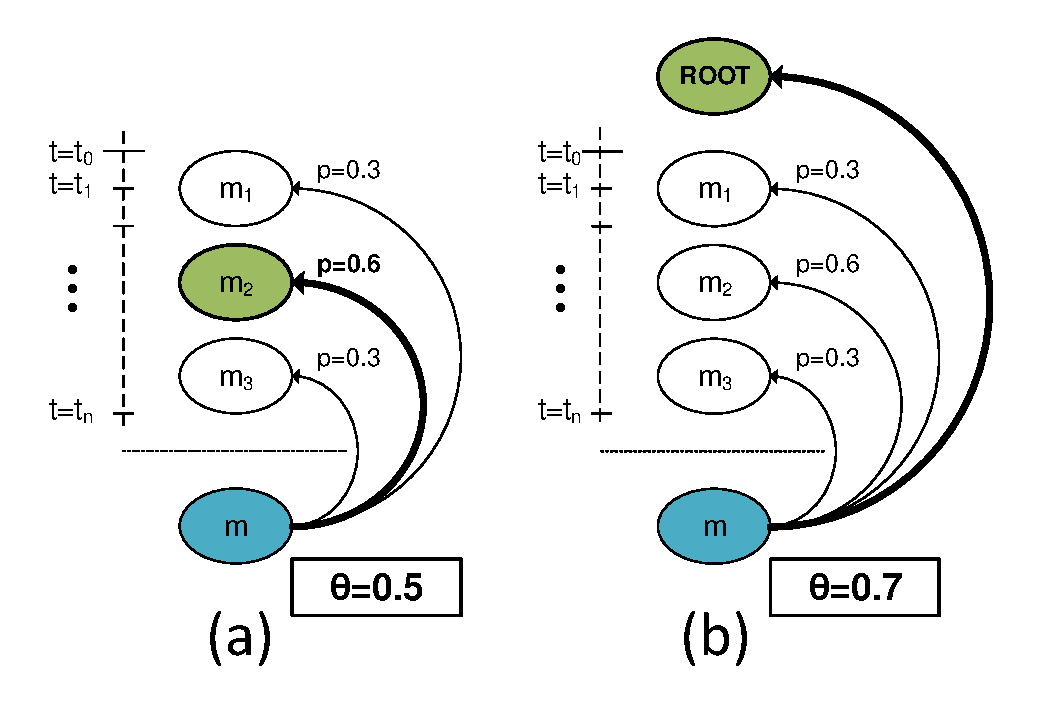
\includegraphics[width=0.65\textwidth]{attachment.pdf}
  \caption{The attachment approach used in our model. We define a probability threshold, 
  $\theta$, and then calculate the attachment probability between a candidate
  node and all preceding nodes in the timeline from the beginning of time.
  Then, for the node for which we obtain maximum attachment probability, we
  may (a) attach the candidate if the probability exceeds the threshold, or
  (b) attach to root by default.}
  \label{fig:treemaker}
\end{figure*}

\subsection{Evaluating classification accuracy}
\label{sec:evaluation}
In evaluating how closely our system reconstructs the original tree, no single
known metric seems to describe the quality of results completely. For this
reason, we use multiple scoring methods in our presentation of results.

Since the task of our system is to guess the parent of each message, a natural
measure of accuracy is F1, computing the precision and recall on the count of
correctly guessed $(parent,child)$ conversation edges against the gold tree.
We present two versions of F1, ``tree F1'', where precision and recall are
calculated based on counts over all messages, and ``average F1'', where
individual F1 scores are calculated for each conversation tree, then averaged
to find the final F1.

Qualitatively speaking, tree F1 reflects how accurately the system makes
individual guesses, while average F1 describes how accurate the predicted
trees are. Since the difficulty of the problem scales with the size of the
conversation, Average F1 will be more forgiving depending on the variance of
conversation sizes in the dataset. With no variation in size, the measures
would be exactly the same.

\subsection{Evaluating subconversation clustering accuracy}
While the ability of the classifier to completely reconstruct a conversation
tree is certainly the ideal scenario, we would also like to see its ability to
preserve the general discourse stucture at a macroscopic level. A typical
online conversation begins with a central message, followed by multiple
primary replies, which then set off a series of subconversations with shorter
and more localized responses. In general, we want to be able to detect that a
group of messages belong to the same \emph{subconversation}, without
particularly concerning ourselves with individual message attachments.

This intuition motivates the choice of a clustering accuracy metric that
compares the set of messages between subconversations of the gold and guess
trees. For this paper, we use the B-CUBED clustering metric \cite{Bagga98} and
obtain average F1 scores across subconversations.

To cluster the messages, we start at a specified depth and, for each message
at that depth, we obtain the set of its children. We do this for both the
guess and the gold trees, and as a result, obtain two different partitions of
the same messages. We discard any messages that belong to either the gold
partition but not the guess partition (or vice versa), which could happen if
those messages were attached at a lower depth in either the guess or gold
partitions than the depth under consideration.

With the two gold and guess partitions of messages, we calculate the B-CUBED
precision, recall and F1 score, as described in \newcite{Bagga98}. We perform
this evaluation at depths of 1, 2, 3 and 4 in order to study the change in
clustering accuracy as we delve deeper into smaller, more localized
conversations.

\subsection{Features}
\label{sec:features}
We decided to try out a split of semantic and non-semantic features to see how
well we could reconstruct trees. To quantify our progress, Table
\ref{table:perfeature} shows the results of a naive bayes classifier trained on
each feature \textit{in isolation}. Below, we describe all the features and
attempt to interpret our results. 

There is a dichotomy between features that tend to benefit attachment to the
root (top level discussion) and features that tend to benefit messages lower
down in the tree. In general, we found that most of the ``low hanging fruit''
non-semantic features seem to discriminate well underneath the root, while
more complicated semantic features (TF-IDF, LDA) seem to get most of their
benefit deeper. This seems to suggest that \textit{post similarity} is more
discriminating lower in the tree, or that sub-discussions veer off the topic
of the main discussion.

\begin{table}[ht]\footnotesize
 \begin{tabular}{| l | l | l | l | l | l | l |} 
   \hline
   \textbf{Feature} & \multirow{2}{*}{\shortstack{Tree\\*F1}} & \multirow{2}{*}{\shortstack{Avg.\\*F1}} & \multicolumn{4}{c|}{$B^3$ depth} \\
                      & & & 1 & 2 & 3 & 4\\
   \hline
   %All-reply-to-root Baseline & 0.476 & 0.488 & 0.641 & & & \\
        %Linear-reply Baseline & 0.093 & 0.111 & 0.219 & 0.178 & 0.144 & 0.125 \\
      Hour Difference & 0.28 & 0.29 & 0.51 & 0.31 & 0.24 & 0.24 \\
   % I'm guessing this reflects some property of the sort algorithm they use
               TF-IDF & 0.31 & 0.32 & 0.44 & 0.48 & 0.44 & 0.41 \\ 
   % This indicates that TF-IDF is mostly helpful in sub-discussions, which is interesting
       Author Mention & 0.46 & 0.48 & 0.64 & 0.07 & 0.07 & \\
   % This indicates author mentions are really only useful at top level, which is interesting
        Reply to Self & 0.48 & 0.50 & 0.63 & 0.21 & & \\
   % Indicates people reply to themselves at the top level rarely, but sometimes lower in the tree
Named Entities & 0.44 & 0.46 & 0.64 & 0.12 & 0.12 & 0.16 \\
   % Kind of contrasts to the TF-IDF feature, people only talk about similar entities high in the tree?
               LDA Divergence & 0.15 & 0.16 & 0.32 & 0.39 & 0.41 & 0.39 \\
   % Sort of like similarity, starts off weak but picks up deeper into the discussion
   % Always weaker than similarity. Probably correlated.
         Flesch-Kincaid & 0.14 & 0.16 & 0.37 & 0.36 & 0.35 & 0.33 \\
   % Pretty much a "for funzies" feature. Interesting that it predicts more in sub-discussions
            Poster Reputation & 0.15 & 0.17 & 0.36 & 0.34 & 0.36 & 0.41 \\
   % Increases as we go down in depth
   \hline
  \end{tabular}
  \caption{Development Set Scores on AskHN data for naive bayes run exclusively
  on a single feature}
  \label{table:perfeature}
\end{table}

\paragraph{Hour Difference} This feature is the number of hours between a parent 
post timestamp and a child timestamp. This appears to have a modest impact on
at all depths of the tree.

\paragraph{TF-IDF} The cosine-similarity between parent post and child. We compute the 
TF-IDF weighting with each message in a tree as a document (i.e. we get a new
weighting scheme for every tree). This was our most helpful \textit{semantic}
feature and gives a large boost to performance. In contrast to many other
features, the performance boost seems to be more pronounced at higher depths
in the tree. We remark that this is actually insightful - cosine similarity of
text becomes more pertinant as discussions get more specialized. This confirms
our hypothesis that sub-discussions actual contains their topics in
themselves.

\paragraph{Author Mention Feature} A 0/1 feature identifying whether the child 
post mentions the parent's author. As Table \ref{table:perfeature} shows, this
fires very rarely but with high precision. Interestingly, we notice that data
gets sparser as the depth increases - this indicates that people are less apt
to mention their parent's name as discussions descend into sub-discussions.

\paragraph{Reply to Self Feature} Whether both parent and child have the same
author. Again, this is a high-precision feature that indicates whether a
person is in reply to themselves (which happens rarely in the data). We notice
that this feature is able to make high-precision decisions at depth 1 and
depth 2, which is likely due to sparsity of data as the discussion descends.

\paragraph{Named Entity Jacard Feature} This feature breaks up Stanford parsed NER
entities (LOCATION, PERSON, ORGANIZATION and MISC) and compares the Jacard
Similarity of the parent post and child. We compute separate features for each
type of entity. We notice that this feature gets a high score near the top of
the tree but a very low score as  discussions descend downwards. As such, it
would appear people are more prone to mention named entities that occur in the
root node then appear in sub-discussions. Many of the AskHN posts revolve
around topics such as ``Where is your startup located?'' and which puts our
results in context.

\paragraph{LDA Divergence} Here we compute the KL-Divergence of the topic distribution
of parent and child. We calculated the topic distribution using 20 topics with
an $\alpha=\frac{5}{2}$ and $\beta = 0.5$. One of the intersting findings is
that LDA appears to be dramatically more useful in classification in higher
depth decisions than near the top of the tree, where it performs abysmally
(0.14 pairwise F1 score). This requires more investigation - our initial
hypothesis is that topics (such as start-ups, or work) are more discriminative
as discussions tend towards sub-discussions. It seems probable that the top-
level discussions all revolve around the same discussion.

\paragraph{Flesch-Kincaid} This is the Flesch-Kincaid readability score. We computed
two features - the parent's score by the child's score and the child's score
divided by the parent. We included this feature ``for fun'' to see whether it
would give us any interesting non-semantic correlation between a poster's
vocabularly and that of the child. From Table \ref{table:perfeature}, this
doesn't appear to show any interesting correlations.

\paragraph{Poster Reputation} Here, we calculated the reputation or ``karma'' of the
parent poster and divided it by the ``karma'' of the child poster. We did the
same for the child divided by the parent. Like many features, this did not
appear to be particularly discriminative - we suspect that there is not a
clear pattern between high karma users and low karma users interacting. At
most, the signal appears to be lower in the tree rather than higher in the
tree. More investigation needs to be performed to determine whether average
karma varies wih depth.


\section{Results}
\label{sec:results}
We used the popular software Weka \cite{Weka2009} and Mallet \cite{McCallum2002Mallet}.
Lorem ipsum dolor sit amet, consectetur adipisicing elit, sed do eiusmod
tempor incididunt ut labore et dolore magna aliqua. Ut enim ad minim veniam,
quis nostrud exercitation ullamco laboris nisi ut aliquip ex ea commodo
consequat. Duis aute irure dolor in reprehenderit in voluptate velit esse
cillum dolore eu fugiat nulla pariatur. Excepteur sint occaecat cupidatat non
proident, sunt in culpa qui officia deserunt mollit anim id est laborum.

\begin{table}[ht]\footnotesize
 \begin{tabular}{| l | l | l |} 
   \hline
   \textbf{Statistic} & Pairwise F1 & Average-tree F1 \\
   \hline
    SVM baseline & 0.329 & 0.331 \\
    All-reply-to-root baseline & 0.278 & 0.278 \\
    One-thread baseline & 0.021 & 0.021 \\
   \hline
  \end{tabular}
  \caption{Data statistics of our preliminary conversation dataset}
  \label{table:results}
\end{table}

\section{Error Analysis}
%TODO
We should put something here.

\section{Conclusion and Next Steps}
Throughout our work, we have tried to address the fundamental question of how
discussion evolves in an online setting. As a way of answering this question,
we proposed the task of \textit{thread reconstruction} on modern online forums
such as Hacker News and Reddit. Disentanglement has a number of user-facing
applications. One might imagine a system that induces tree structure out of
flat conversations to make email chains and chat rooms more readable. Building
an effective model for this problem is interesting also because we can compare
performance with various sets of features to gain insight into how tree-
structured online discourse evolves.

In our feature engineering experiments listed in Section \ref{sec:features} we
found an interesting divide between features that primarily benefit high-depth
attachments, and features that primarily benefit root-level attachments. This
suggests that finding the correct balance of features may require us to take
into account \textit{previous} decisions we made in our classification tree.
Although we are not yet experienced in the realm of probabilistic graphical
models, we believe our work leads to a natural extension using conditional
random fields (CRFs) to factor in all possible tree decision structures, as
opposed to taking taking a greedy approximation. In addition to a better
balance, CRFs would allow us to factor in features that extend beyond the
$(parent,child)$ relationship such as parent depth, grand parent mentions, our
cluster topics.

Although LDA was unable to capture \textit{speech acts} as a feature, much of
the literature mentioned in Section \ref{sec:prior_work} suggests that they
may be a key component in understanding dialog structure. After gaining some
more experience with graphical models, we would like to revisit our data and
see if we can find an LDA-like act that could explain some of the reply
relationships. As our analysis showed

As an extension to our evaluative measures, we suspect that there is an upper
bound to human-level performance on this task. Often, replies online are short
and without context (e.g., ``I had the same idea'', or ``That's awesome!'').
Although speech acts may help understand some of the structure, it is probable
that humans would also have difficulty attaching messages to the root. We
propose a future experiment utilizing Amazon's Mechanical Turk to perform
conversation reconstruction with real humans. This would provide us an upper
bound on our performance and give our models something to aim for in terms of
our proposed evaluation metrics.

Our CS224U project has been a learning experience for all of us. We are
particularly pleased with the domain we uncovered and dataset that we have
captured. As noted in Section \ref{sec:evaluation}, our evaluation
measurements help quantify how well we preserve conversation \textit{order} as
well as how we preserve the general discourse. Obviously, the experiments have
piqued our curiosity about the nature of conversation. In the near future, we
hope to revisit our questions with armed with machinery of graphical models.

\bibliography{final_report}{} 
\bibliographystyle{acl2012}

\end{document}
